\documentclass[First Project.tex]{subfiles}
\begin{document}

\subsection{ Αποσύνθεση \textlatin{\textbf{Cholesky}} }

Η μέθοδος της αποσύνθεσης \textlatin{\textbf{Cholesky}} αφορά συμμετρικούς και θετικά ορισμένους $n \times n$ τετραγωνικούς πίνακες τους 
οποίους αποσυνθέτει στο παρακάτω γινόμενο 
\begin{equation*}
    R^{T}R , 
\end{equation*}
με τον $R$ να είναι άνω τριγωνικός. Η συνάρτηση που έχει υλοποιηθεί στο αρχείο \textlatin{\textbf{cholesky\_decomposition.py}} υλοποιεί τον 
παρακάτω αλγόριθμο :
\begin{itemize}
    \item Για κάθε γραμμή $i$ του πίνακα $Α$ αν το στοιχείο $A_{ii}$ είναι αρνητικό ο αλγόριθμος σταματάει.
    \item Ανάθεσε στο στοιχείο $R_{ii}$ την τετραγωνική ρίζα του $A_{ii}$.
    \item Βρες τον διάνυσμα $u^{T}$ σύμφωνα με το $u^{T} = \frac{1}{R_{ii}} * A_{i,i+1:n}$
    \item Τοποθέτησε το διάνυσμα $u^{T}$ στα στοιχεία δεξιά της κύριας διαγωνίου στην γραμμή $i$ σύμφωνα με το $R_{i,i+1:n} = u^{T}$  
    \item Αφαίρεσε από τον διάστασης $i+1$ υποπίνακα του $Α$ τον πίνακα $uu^{T}$ σύμφωνα με το $A_{i+1:n,i+1:n} = A_{i+1:n,i+1:n} -uu^{T}$ 
\end{itemize}

Πιο συγκεκριμένα, η συνάρτηση \textlatin{\textbf{chol}} δέχεται ως παράμετρο τον πίνακα \textlatin{A} και επιστρέφει τον κάτω τριγωνικό πίνακα
$L$ ( ή τον $R^{T}$ ) που αποτελεί την αποσύνθεση \textlatin{\textbf{Cholesky}} του πίνακα \textlatin{A}. Αρχικά, η συνάρτηση πραγματοποιεί 
τις κατάλληλες αρχικοποιήσεις για τον πίνακα $R$ και δημιουργεί ένα αντίγραφο του πίνακα $A$ έτσι ώστε να μην πραγματοποιήσει
καμία αλλαγή στον πίνακα που πήρε σαν όρισμα. Στην συνέχεια, για κάθε γραμμή $i$ του αντίγραφου του πίνακα $A$ ελέγχει αν $A_{ii} < 0 $ και αν
ναι, η συνάρτηση σταματάει και επιστρέφει τον ανάστροφο πίνακα του $R$. Αν όχι η συνάρτηση συνεχίζει και αναθέτει στο στοιχείο $R_{ii}$ το
$\sqrt{A_{ii}}$. Στην συνέχεια, υπολογίζεται το διάνυσμα $u^{Τ}$ και αντιγράφονται τα στοιχεία του στα δεξιά του στοιχείου $R_{ii}$. Τέλος, 
υπολογίζεται ο πίνακας $uu^{T}$ και αφαιρείται από τον $i+1$ διάστασης υποπίνακα του $Α$. Στην συνέχεια, παρουσιάζεται ένα παράδειγμα εύρεσης
της αποσύνθεσης \textlatin{\textbf{Cholesky}} με την χρήση της συνάρτησης \textlatin{\textbf{chol}} με το οποίο τελειώνει αυτή η παράγραφος.
Στο παράδειγμα μας ο πίνακας $Α$ είναι ο  
\begin{center}
$A = \begin{pmatrix}
9 & 0 & -27 & 18 \\
0 & 9 & -9 & -27 \\
-27 & -9 & 99 & -27 \\
18 & -27 & -27 & 121
\end{pmatrix}$
\end{center}

\vspace{5px}
Για την εύρεση της αποσύνθεσης \textlatin{\textbf{Cholesky}} του παραπάνω πίνακα αρχικά δημιουργούμε τον πίνακα $Α$ με παρόμοιο τρόπο όπως στην
παράγραφο \textbf{4.1} και καλούμε την συνάρτηση \textlatin{\textbf{chol}} με όρισμα τον πίνακα $Α$ από την οποία παίρνουμε τα εξής αποτελέσματα:
\begin{figure}[h!]
    \centering
    \captionsetup{justification=centering}
    \begin{center}
        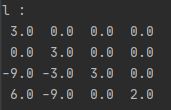
\includegraphics[scale=1]{exercise_3_cholesky_l_matrix.png}    
        \caption{ Αποσύνθεση \textlatin{\textbf{Cholesky}} για τον πίνακα $Α$ }
    \end{center}
\end{figure} 
\end{document}